% v7 --- reframe of the Apex/Dresser case as non-adjudicating; argument reweighted to the
% cross-formation pattern; cross-formation scatter figure reintroduced; experimental and analytical
% programme added. Compile: pdflatex twice.
\documentclass[11pt]{article}
\usepackage[a4paper,margin=2.2cm]{geometry}
\usepackage[utf8]{inputenc}
\usepackage[round,authoryear]{natbib}
\usepackage{booktabs,amsmath,amssymb,mhchem,graphicx,caption,microtype,setspace,array}
\usepackage{tikz}\usetikzlibrary{arrows.meta,positioning,fit,backgrounds}
\setstretch{1.03}
\captionsetup{font=small,labelfont=bf}
\title{\vspace{-1.0cm}\textbf{Early mineral entombment as a taphonomic confound in the
post-Great Oxidation Event microfossil record}}
\author{[Author Name]\\
\small\textit{[Affiliation]}}
\date{}
\begin{document}
\maketitle

\begin{abstract}
\noindent The proposition that an apparent evolutionary radiation may reflect the opening of a
preservational window is well established for the Proterozoic--Cambrian boundary, but has been less
developed across the Great Oxidation Event (GOE; $\sim$2.4~Ga), where the diversification of
morphologically diagnostic microfossils is usually read as biological. We evaluate the hypothesis
that early mineral entombment, predominantly silicification with which early iron mineralisation is
associated, is a taphonomic confound in the post-GOE pattern, against the published petrographic and
geochemical record of seven chert-hosted biotas spanning the GOE, including the 2.45--2.21~Ga Turee
Creek Group. Within the 1.88~Ga Gunflint biota, morphospecies that retain cellular contents carry
$10^{8}$--$10^{9}$ intracellular Fe atoms~$\mu$m$^{-3}$, but this iron may reflect in vivo
biomineralisation, so the observation supports the principle that fidelity requires mineralisation
before decay without isolating silica, though the within-Gunflint correlation is confounded by
wall-recalcitrance and the less confounded comparison is the cross-formation pattern, in which silicification
varies at the facies level independently of morphotype. The hypothesis is then examined against its
best available candidate, the early-silicified but contested Apex and Dresser cherts; this case
cannot adjudicate the hypothesis, because their biogenicity is itself contested and is upstream of
the fidelity question, but the examination exposes a deeper consequence, that silicification
preserves morphology indiscriminately, entangling fidelity with biogenicity. We state explicitly
the two conditions that would falsify the hypothesis. We note that the biomarker evidence for pre-GOE eukaryotes is best regarded as
contaminant, while the obligate aerobicity of sterol biosynthesis gives eukaryotes a
mechanistically independent reason to diversify with oxygen. The post-GOE ``rise'' of microfossils
therefore plausibly reflects, in part, a facies-controlled preservational signal, but the partition
between evolution and unmasking is unresolved and lineage-conditional. The paper advances a
hypothesis; it reports no new measurements.
\end{abstract}

\noindent\textbf{Keywords:} Great Oxidation Event; taphonomic megabias; silicification; iron
mineralisation; Archaean--Proterozoic; microfossils; molecular clocks; sterol biosynthesis.

\section{Introduction}

It has long been recognised that anoxia retards the degradation of sedimentary organic matter, and
that the destruction of cellular morphology during early decay proceeds more slowly where molecular
oxygen is scarce \citep{Canfield1994,Hedges1995}. From this premise the Archaean ocean, in which
dissolved oxygen was negligible \citep{Pavlov2002} and sulfate scarce \citep{Habicht2002,Crowe2014},
might be expected to have favoured the preservation of organic-walled microfossils. The rock record
appears to say the opposite: assemblages of taxonomically diagnostic microfossils become abundant
and widespread only after the GOE \citep{Javaux2018,Wacey2014}.

The proposition that an apparent radiation can reflect the opening of a preservational window rather
than a biological event is the foundation of the taphonomic-megabias literature. \citet{Allison1993}
first quantified the non-random, secular distribution of soft-bodied preservation through the
Phanerozoic, and \citet{Butterfield2003} argued that the distribution of Burgess-Shale-type
preservation constitutes a megabias across the Cambrian explosion. Comparable arguments have been
made for phosphatisation windows in the Ediacaran Doushantuo biota and for silicification in the
Ediacaran \citep{Tarhan2016}. This framework is long established at the Proterozoic--Cambrian
boundary; it has been less developed across the GOE.

The contribution of the present paper is therefore not the megabias concept but its specific
extension to the GOE microfossil record, using the 2.45--2.21~Ga Turee Creek Group as a bridging
case, and paired with a biochemical counterargument, the obligate aerobicity of sterol synthesis,
that bears differentially on eukaryotes. The paper advances a hypothesis and reports no new
measurements; the supporting data are semi-quantitative and drawn from a literature dominated by a
few research groups, a limitation stated explicitly below.

\section{Background}

\subsection{Redox across the GOE}

The disappearance of mass-independent sulfur isotope fractionation between $\sim$2.45 and 2.32~Ga
marks the GOE \citep{Holland2006,Bekker2004,Pavlov2002,Farquhar2000}; the transition was protracted
and regionally diachronous \citep{Lyons2014,Philippot2018}. Iron speciation indicates anoxic,
ferruginous deposition throughout the Archaean and much of the Proterozoic
\citep{Canfield1998,Poulton2005,Poulton2011}, euxinia being spatially restricted
\citep{Reinhard2009}. Seawater sulfate rose across the GOE \citep{Habicht2002,Kah2004,Crowe2014},
but sulfur isotope evidence of this rise extends into the Neoarchean \citep{Reinhard2009}, and
signals of oxidative weathering precede the GOE in several basins \citep{Anbar2007}.

\subsection{The microfossil record and the Turee Creek Group}

The Archaean record of cellular morphology is sparse and contested. The $\sim$3.46~Ga Apex chert
filaments \citep{Schopf1993} were reinterpreted as abiogenic \citep{Brasier2002}, and although
better-preserved Archaean microbiotas are known from the $\sim$3.4~Ga Strelley Pool Formation
\citep{Sugitani2010,Delarue2020}, their cellular fidelity is modest. The most directly relevant
succession is the Turee Creek Group ($\sim$2.45--2.21~Ga), which spans the GOE and preserves diverse
microfossil communities in black chert \citep{Barlow2018}, the taphonomy and iron mineralisation of
which are documented by \citet{Lepot2017b}. Gunflint-type biotas of $\sim$1.9~Ga age carry
filaments, spheroids and spindle-shaped forms in cellular detail \citep{Lepot2017a,Javaux2018}.

\subsection{The silica cycle}

Before the evolution of silica-biomineralising organisms the ocean was saturated with respect to
amorphous silica, with dissolved concentrations of order $\sim$2~mM and abiological precipitation
the dominant sink \citep{Siever1992,Perry2007}. The capacity for early silica precipitation was
therefore available on both sides of the GOE; silica was not drawn down until the much later
radiation of sponges, radiolaria and diatoms.

\subsection{A biochemical oxygen constraint on eukaryotes}

Sterol biosynthesis is obligately aerobic: the cyclisation and oxidative modification of squalene
requires molecular oxygen, on the order of eleven molecules of \ce{O2} per sterol
\citep{Gold2017,Desmond2009}. Crown eukaryotes synthesise sterols, and the last eukaryotic common
ancestor is inferred to have done so \citep{Desmond2009}. This provides a mechanistically independent
reason to expect crown-eukaryote diversification to track the availability of oxygen, though
molecular-clock estimates of when that diversification occurred are themselves partly calibrated to
GOE geochemistry \citep{Gold2017}, so the independence that holds is biochemical rather than
chronological.

\section{Material and approach}

Seven chert-hosted biotas were compared (Table~\ref{tab:panel}): Strelley Pool, Moodies and Tumbiana
(pre-GOE), the Turee Creek Group (which spans the GOE), and the Belcher Group, Gunflint and Sokoman
(post-GOE). These are the principal GOE-adjacent silicified biotas in the literature; the selection
is practical rather than the product of a formal survey, and the candidate that might have served as
a sharp test is examined in Section~\ref{sec:falsify}. The units span shallow-marine to peritidal
silicified facies of comparable, low metamorphic grade. For each, published petrography, Raman
spectroscopy, iron mineralogy and sulfur geochemistry were compiled; no new measurements are reported.

To reduce circularity, the degree of early silicification is assessed from criteria independent of
the fidelity outcome: the timing of silica cementation relative to compaction fabrics (pre-compaction,
wall-conforming microquartz or chalcedony indicating early entombment, versus late megaquartz
void-fill) and the quartz cement fabric. These criteria, and the unit to which each applies, are
given in Table~\ref{tab:panel}.

The independence of these criteria from the fidelity outcome is logical rather than source-based.
The petrographic assessments and the fidelity assessments alike are drawn from a literature dominated
by a few overlapping research groups (principally Lepot, Javaux and Wacey), so the compiled comparison
cannot be treated as source-independent, and the criteria-scored cross-formation plot
(Fig.~\ref{fig:scatter}) is illustrative rather than a formal test. This limitation is restated and
developed in the Discussion, where it bounds the strength of the claim.

\begin{table}[t]
\centering\small
\caption{Preservation of cellular morphology in seven chert-hosted biotas, with the petrographic
criterion used to assess the timing of silicification, kept separate from the fidelity outcome.}
\label{tab:panel}
\begin{tabular}{p{0.15\linewidth}p{0.09\linewidth}p{0.27\linewidth}p{0.27\linewidth}p{0.10\linewidth}}
\toprule
Unit (age) & GOE & Silicification criterion (independent of fidelity) & Preservation of morphology & Source \\
\midrule
Strelley Pool ($\sim$3.4~Ga) & pre & early silicification; wall organic matter partly replaced by microquartz/chalcedony & diverse (lenticular, spinose) but lower cellular fidelity than Gunflint & \citep{Sugitani2010,Delarue2020,Wacey2012} \\
Moodies Gp ($\sim$3.22~Ga) & pre & silicification of mat textures only; cells not encapsulated & tufted, cavity-dwelling mats; cellular detail poorly resolved & \citep{Homann2015} \\
Tumbiana Fm ($\sim$2.72~Ga) & pre & organic matter hosted in carbonate; cells not silica-encapsulated & kerogenous globules; rare filaments & \citep{Lepot2009,Decraene2021} \\
Turee Creek Gp ($\sim$2.45--2.21~Ga) & spans & early chert permineralisation with associated Fe mineralisation & diverse spheroids and filaments across the GOE & \citep{Lepot2017b,Barlow2018} \\
\midrule
Belcher Gp ($\sim$2.0~Ga) & post & chert replacement of stromatolitic carbonate & diverse microbiota, chert-permineralised & \citep{Javaux2018} \\
Gunflint Fm ($\sim$1.88~Ga) & post & pre-compaction silica encapsulation; intra-microfossil microquartz finer than matrix & diverse, high cellular fidelity; intra-cellular Fe-silicate/carbonate & \citep{Lepot2017a,Wacey2013,Alleon2016} \\
Sokoman IF ($\sim$1.88~Ga) & post & early chert of iron-formation & Gunflint-type assemblage & \citep{Javaux2018} \\
\bottomrule
\end{tabular}
\end{table}

\section{Evidence}

\subsection{A within-assemblage covariation, and its interpretation}

Within the Gunflint biota, the preservation of internal cellular structure is coupled to early
mineralisation. Morphospecies retaining cellular contents carry between $3\times10^{8}$ and
$10^{9}$ intracellular Fe atoms~$\mu$m$^{-3}$, with intra-microfossil quartz finer than the
surrounding matrix; empty sheaths remain at the chert background
($\sim$$1.5\times10^{6}$~atoms~$\mu$m$^{-3}$; Fig.~\ref{fig:gunflint}) \citep{Lepot2017a}.

This correlation carries a caveat that bears directly on the argument. \citet{Lepot2017a} interpret
the intracellular iron as consistent with in vivo biomineralisation, plausibly by oxygenic
photosynthesisers, rather than as a purely external precipitate. If so, the mineral phase associated
with fidelity is partly a metabolic product, and the opposition between preservation and biology is
less clean than a taphonomic reading would prefer. The observation nevertheless establishes the
principle that fidelity required mineralisation before decay. It does not isolate silica as the
agent; the assignment of silicification as the entombment medium rests on silica-specific evidence:
the three-dimensional preservation of Gunflint cells within quartz, requiring silica encapsulation
before compaction \citep{Lepot2017a,Alleon2016}, and wall-conforming microquartz more generally
\citep{Wacey2012}.

A second, structural confound limits what the within-Gunflint correlation can establish. The
morphospecies that retain cellular contents are thick-walled forms, and wall recalcitrance and the
capacity to nucleate intracellular minerals are co-varying properties of the morphotype rather than
independent consequences of entombment timing. The within-Gunflint covariation is therefore
suggestive but cannot, by itself, distinguish entombment timing from morphotype recalcitrance as the
cause. It is consequently treated here as supporting rather than flagship evidence; the less confounded comparison
is the cross-formation pattern of the next subsection, where silicification varies at the facies
level and is independent of morphotype (see also Discussion).

\begin{figure}[t]
\centering
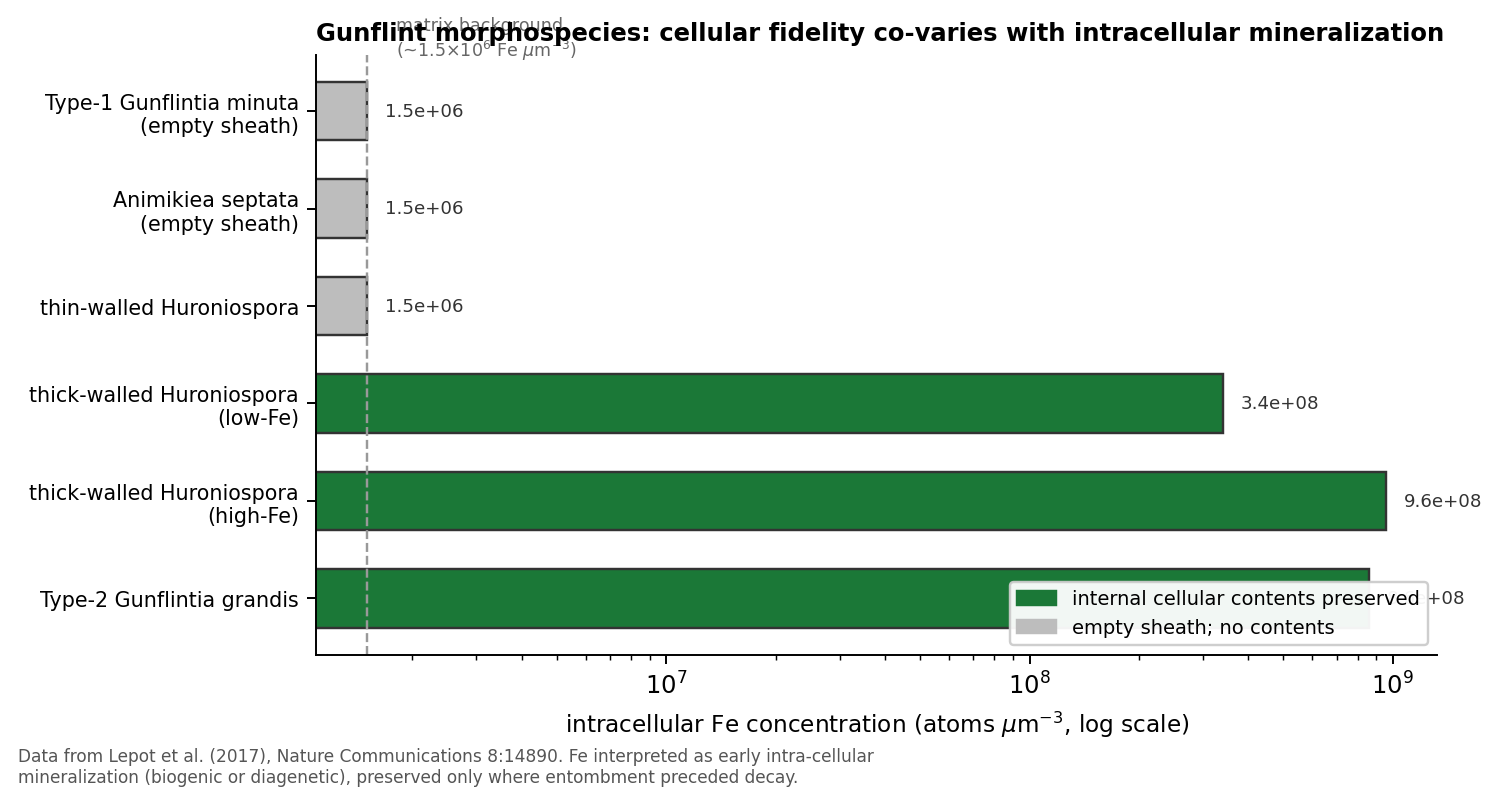
\includegraphics[width=0.92\linewidth]{fig_gunflint.png}
\caption{Intracellular Fe concentration in Gunflint morphospecies, against the preservation of
cellular contents. The iron may reflect in vivo biomineralisation \citep{Lepot2017a}, so the
covariation links fidelity to early mineralisation without isolating silica as the agent. Data from
\citet{Lepot2017a}.}
\label{fig:gunflint}
\end{figure}

\subsection{The between-assemblage pattern}

The cross-formation comparison provides the more compelling illustration of the hypothesis, and for a specific
reason: across the seven units, variation in silicification operates at the facies level, across
units of differing lithology and depositional setting, and is therefore independent of the
morphotype-specific recalcitrance that confounds the within-Gunflint correlation. Where silicification
was early and complete, cellular morphology is preserved; where it was weak or absent, only kerogen
and mats survive.

Across the seven units, the preservation of cellular morphology tracks the independent indicators of
early silicification rather than position relative to the GOE (Table~\ref{tab:panel};
Fig.~\ref{fig:scatter}). The pre-GOE Strelley Pool biota preserves a diverse assemblage, albeit with
lower cellular fidelity than Gunflint \citep{Wacey2012}; the pre-GOE Tumbiana and Moodies biotas
preserve kerogen and mats rather than cells \citep{Lepot2009,Homann2015}; the Turee Creek Group,
which spans the GOE, preserves diverse silicified microfossils with associated iron mineralisation
\citep{Lepot2017b,Barlow2018}, a pattern continuous across the boundary rather than stepped at it;
and the post-GOE Gunflint, Sokoman and Belcher biotas are early-silicified and morphologically rich
\citep{Lepot2017a,Javaux2018}. Pyrite is a poor indicator of fidelity: pyritisation is patchy and
destructive in Gunflint \citep{Wacey2013,Lepot2017a} and is documented in pre-GOE Tumbiana
stromatolites \citep{Decraene2021}. Plotted as a coarse fidelity-versus-silicification scatter
(Fig.~\ref{fig:scatter}), the seven biotas fall close to a 1:1 relationship, consistent with
silicification governing fidelity; the plot is criteria-scored and not source-independent, however,
and is illustrative rather than the formal regression proposed below.

\begin{figure}[t]
\centering
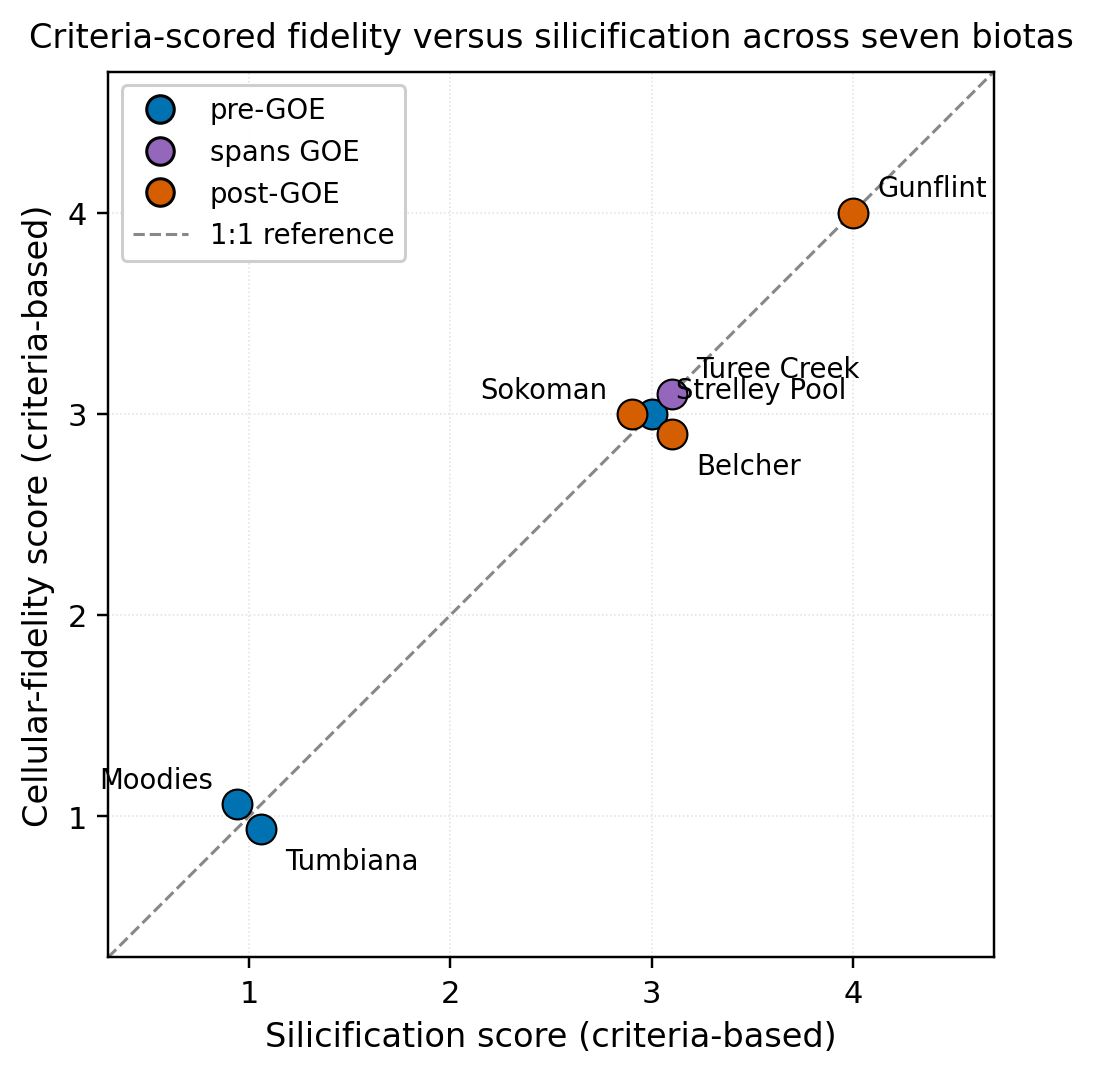
\includegraphics[width=0.82\linewidth]{fig_v7_scatter.png}
\caption{Criteria-scored fidelity versus silicification across seven biotas. Scores are
criteria-based and compiled from the same descriptive literature; they are not source-independent
(see text). The correlation is illustrative, not a formal test. Overlapping points are slightly
offset for visibility. The dashed line is a 1:1 reference.}
\label{fig:scatter}
\end{figure}

\subsection{Why redox and the silica cycle do not supply a GOE control}

Iron speciation indicates pervasive ferruginous deposition on both sides of the GOE
\citep{Canfield1998,Poulton2011}, and the sulfur isotope signal of rising sulfate extends into the
Neoarchean \citep{Reinhard2009,Philippot2018}. The sulfate rise bears on microbial sulfate
reduction and the sulphurisation of organic matter, affecting the survival of bulk kerogen rather
than the templating of cellular morphology. The capacity for early silica precipitation was likewise
unchanging across the GOE \citep{Siever1992,Perry2007}.

\section{A case that cannot adjudicate: pre-GOE silicified cherts}\label{sec:falsify}

The most promising candidate for a sharp test of the hypothesis would be a pre-GOE chert that is
demonstrably early-silicified. The $\sim$3.46~Ga Apex chert and the $\sim$3.48~Ga Dresser Formation
are pre-GOE, silicified, and rich in cell-like carbonaceous structures, and so might appear to
provide exactly such a test. They cannot. The Apex filaments described as microfossils
\citep{Schopf1993} were reinterpreted as abiogenic mineral artefacts \citep{Brasier2002}, and
high-resolution reinvestigation has reinforced an abiogenic, hydrothermal origin for many such
structures \citep{Wacey2014}. Where biogenicity is itself contested, no observation of cellular
fidelity can adjudicate the entombment-timing hypothesis, because the question of whether these
structures were ever cells is logically upstream of the question of how faithfully their morphology
was preserved. A chert of disputed biogenicity is therefore structurally incapable of testing the
hypothesis, and we treat Apex and Dresser as informative about the nature of silicified cherts
rather than as a falsification test that the hypothesis has survived.

The observation these cherts do support is narrower but worth stating plainly. Silicification
preserves morphology indiscriminately --- whether the substrate is biological or abiotic --- so
silicified cherts will contain cell-like structures of mixed origin, and the biogenicity question is
upstream of the fidelity question. The scarcity of unambiguous pre-GOE microfossils is consequently
not evidence that silicification was feeble in the Archaean (it demonstrably was not
\citep{Siever1992,Perry2007}), but that silicification records both biology and abiotic look-alikes,
leaving few structures that meet modern biogenicity criteria. This is a statement about the nature
of silicified cherts, not a falsifier the hypothesis has passed.

What would constitute a genuine test is a chert carrying microfossils of undisputed biogenicity,
with demonstrably early silicification, and varying cellular fidelity. A single such unit in which
early entombment coexisted with poor fidelity would falsify the hypothesis outright. No such case is
presently known: every well-preserved early-silicified biota of accepted biogenicity also preserves
morphology well, and every pre-GOE chert of disputed biogenicity cannot serve as a test for the
reason given above.

\section{Origins, first appearances, and the sterol constraint}

Molecular clocks place the stem origin of cyanobacteria, and oxygenic photosynthesis, in the Archaean
\citep{Fournier2021}, whereas the crown-group diversification of extant Oxyphotobacteria postdates
the rise of oxygen \citep{Shih2017}. Molecular clock estimates for the last eukaryotic common
ancestor are model-dependent but several precede the first widely accepted eukaryotic microfossils
\citep{Betts2018,Eme2014} (Fig.~\ref{fig:clocks}). The biomarker record cannot resolve the resulting
gap: the steranes and 2-methylhopanes reported from $\sim$2.7~Ga shales \citep{Brocks1999} reside in
younger carbonate veins \citep{Rasmussen2008} and are indistinguishable from procedural blanks in
ultraclean cores \citep{French2015}.

\begin{figure}[t]
\centering
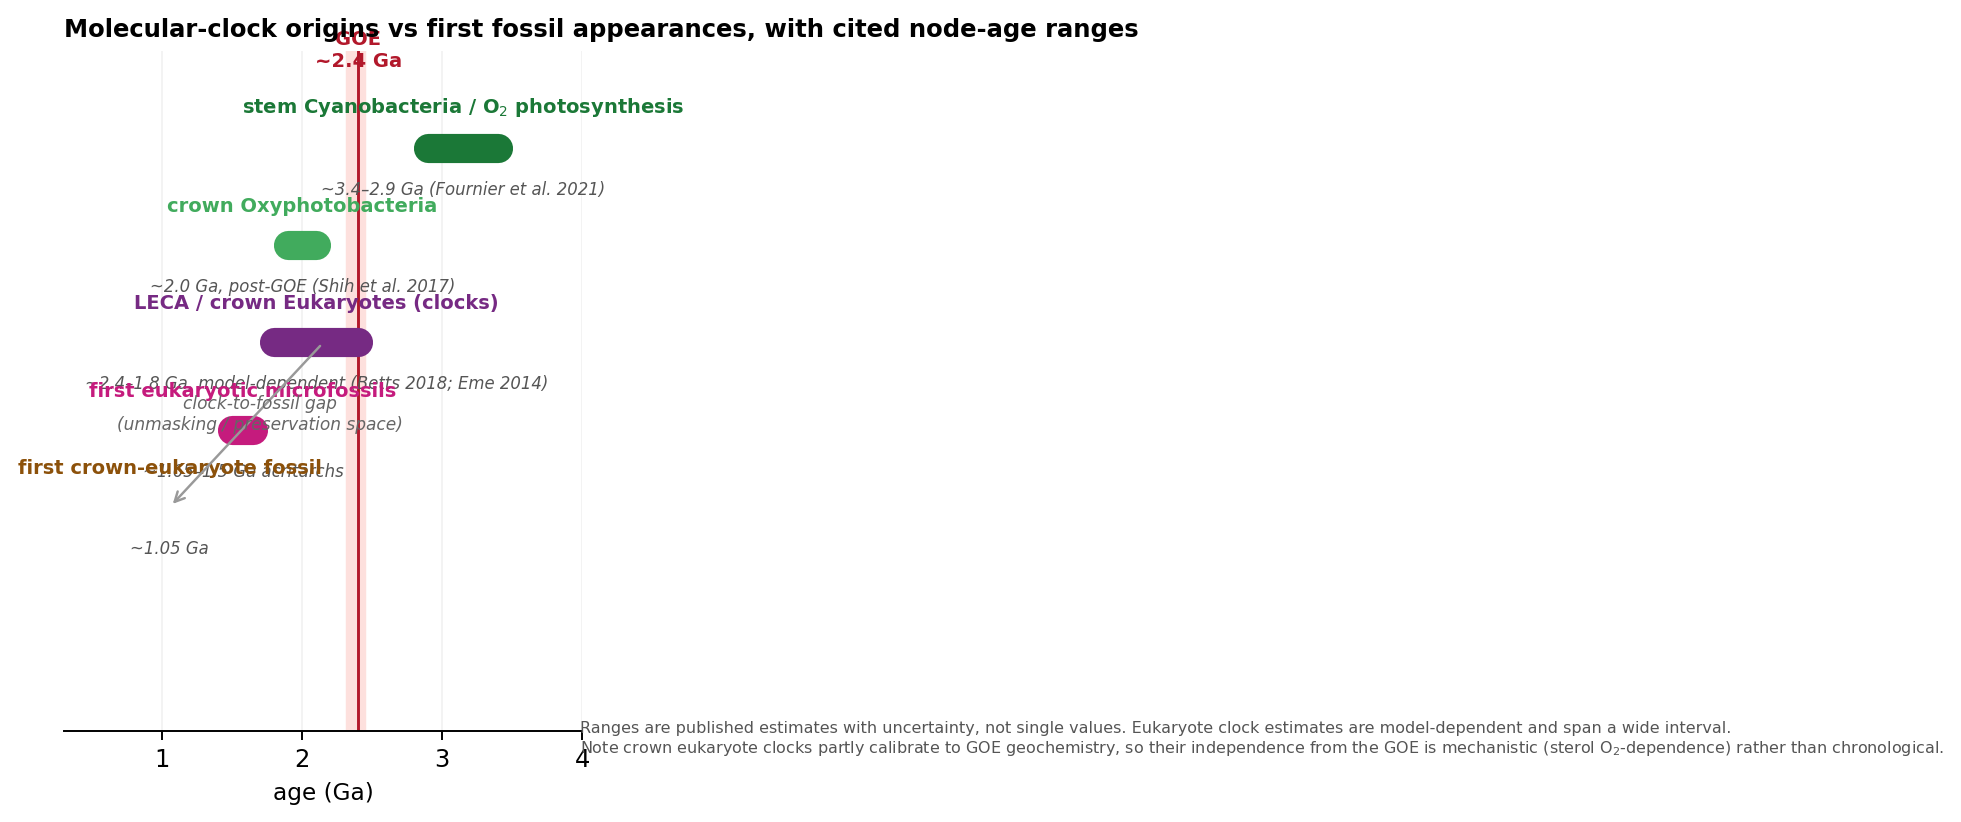
\includegraphics[width=\linewidth]{fig_v6_timeline.png}
\caption{Molecular clock estimates of lineage origin against first fossil appearances, with
published node-age ranges. The stem origin of cyanobacteria lies in the Archaean \citep{Fournier2021};
crown Oxyphotobacteria diversify around or after the GOE \citep{Shih2017}; eukaryote estimates are
model-dependent \citep{Betts2018,Eme2014} and partly calibrated to GOE geochemistry.}
\label{fig:clocks}
\end{figure}

The obligate aerobicity of sterol synthesis \citep{Gold2017,Desmond2009} cuts across a purely
preservational reading for eukaryotes: crown eukaryotes have a mechanistic reason to diversify once
oxygen became available, regardless of preservation. The clock-to-fossil gap for eukaryotes is thus
not necessarily a preservational lag and may reflect genuine, oxygen-limited diversification. The
unmasking hypothesis is consequently better supported for cyanobacteria, whose metabolism clocks to
the Archaean, than for sterol-synthesising eukaryotes, and any reading must be lineage-conditional.

\section{Discussion}

The compiled record is consistent with the hypothesis that early mineral entombment is a
significant confound in the post-GOE microfossil record. The defensible position is narrow. The
preservation of cellular morphology in Precambrian cherts is conditioned by early mineralisation,
predominantly silicification, that operated throughout but was expressed unevenly, depending on
depositional facies and the timing of cementation relative to decay (Fig.~\ref{fig:model}). Where
entombment was early and complete, morphology survives; where it was weak, kerogen and mats remain.
Oxygenation plausibly modified organic-matter decay and kerogen sulphurisation
\citep{Lepot2009,Decraene2021} but did not gate the silicification on which cellular fidelity depends.

\begin{figure}[t]
\centering
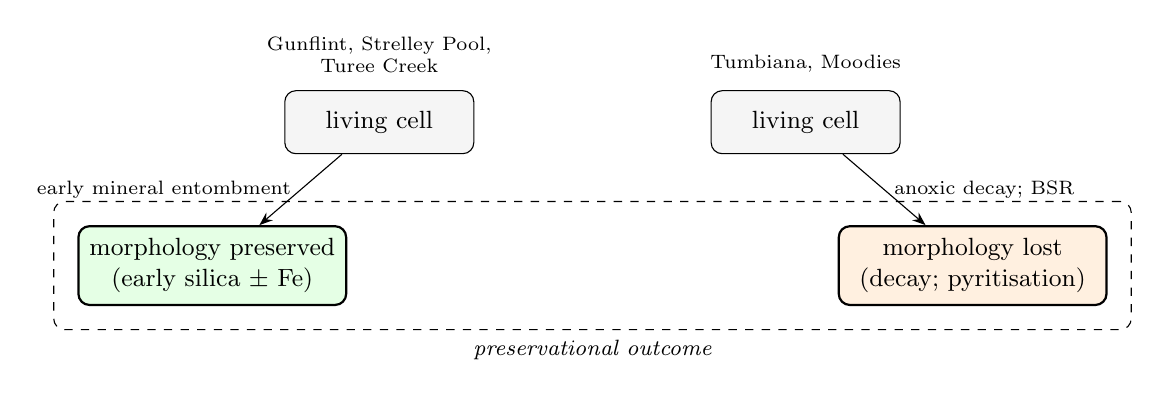
\begin{tikzpicture}[>=Stealth, node distance=6mm and 10mm,
  cell/.style={draw,rounded corners,align=center,fill=gray!8,minimum width=24mm,minimum height=8mm,font=\small},
  outc/.style={draw,thick,rounded corners,align=center,minimum width=34mm,minimum height=10mm,font=\small},
  every node/.style={font=\small}]
\node[cell] (c1) {living cell};
\node[cell,right=30mm of c1] (c2) {living cell};
\node[outc,below left=9mm and -8mm of c1, fill=green!10] (m1) {morphology preserved\\(early silica $\pm$ Fe)};
\node[outc,below right=9mm and -8mm of c2, fill=orange!12] (m2) {morphology lost\\(decay; pyritisation)};
\node[draw,dashed,rounded corners,fit=(m1)(m2),inner sep=3mm,label={[font=\footnotesize\itshape]below:preservational outcome}] {};
\draw[->] (c1) -- node[left,font=\scriptsize]{early mineral entombment} (m1);
\draw[->] (c2) -- node[right,font=\scriptsize]{anoxic decay; BSR} (m2);
\node[above=1mm of c1,font=\scriptsize,align=center]{Gunflint, Strelley Pool,\\Turee Creek};
\node[above=1mm of c2,font=\scriptsize,align=center]{Tumbiana, Moodies};
\end{tikzpicture}
\caption{Preservational pathways. Where early mineral entombment outpaces decay, morphology is
retained; where decay precedes mineralisation, morphology is lost and kerogen survives.}
\label{fig:model}
\end{figure}

The limitations of these compiled observations must be stated plainly, since they define the status of the
contribution. The quantitative correlation rests on a single locality (Gunflint), a single element
(iron), and a single study in which both the mineralisation and the fidelity were documented by the
same authors \citep{Lepot2017a}; the within-assemblage covariation is therefore not
source-independent. A structural confound compounds this: within Gunflint the morphospecies retaining
contents are thick-walled forms, and wall recalcitrance and mineral-nucleation potential are
co-varying properties of the morphotype rather than independent consequences of entombment timing.
This does not rescue a purely biological reading (morphotype-selective preservation is itself a
taphonomic bias) but it means the within-Gunflint evidence cannot, by itself, isolate entombment
timing as the cause. The cross-formation comparison, which uses criteria independent of the fidelity
outcome and varies silicification at the facies level, is the more robust comparison precisely because it
is less susceptible to this confound; but its criteria and fidelity assessments are likewise drawn
from a literature dominated by a few overlapping research groups (principally Lepot, Javaux and
Wacey), so the independence is logical rather than source-based.

The hypothesis would be falsified by (i) a pre-GOE chert bearing confirmed genuine microfossils with
demonstrably early silicification and poor cellular fidelity, or (ii) a within-formation regression
showing no relationship between fidelity and a quantitative silicification index scored blind and
across research groups. Neither is known; both are testable, and the second is achievable with
existing material. The programme needed to pursue them is specified below.

The implications are qualified accordingly. Abundance and diversity counts across the GOE cannot be
read as proxies for biomass without facies correction. The clock-to-fossil gap is consistent with a
preservational lag but, for sterol-synthesising lineages, may equally reflect oxygen-limited
diversification. For the search for ancient biosignatures, the corollary is that the preservation of
morphology requires a silica-precipitating facies rather than the presence of oxygen.

\subsection{What would be needed: an experimental and analytical programme}

The hypothesis is testable; we specify three approaches in order of decisiveness.

\textit{(a) Controlled silicification--decay experiments.} The confound that most limits the
within-Gunflint evidence is the co-variation of wall recalcitrance and mineral-nucleation potential
with morphotype. A laboratory programme can hold morphotype constant and vary only the timing of
silica addition. Microbial cultures spanning thick- and thin-walled morphotypes (e.g.\ cyanobacteria
and other bacteria) would be incubated under factorial O$_2$~$\times$~sulfate~$\times$~Fe conditions,
with controlled silica added at defined intervals after death. Blind-scored cellular fidelity, silica
nucleation timing, and intracellular mineralisation would then reveal whether entombment timing ---
rather than wall recalcitrance --- is the causal variable. Existing experimental work shows that
early entombment within silica minimises the molecular degradation of microorganisms during advanced
diagenesis \citep{Alleon2016silica}, providing a mechanistic basis for the timing effect the
hypothesis predicts.

\textit{(b) A blind, cross-group within-formation regression.} This is the test the present paper
proposes but does not perform. Cellular fidelity and a quantitative silicification index would be
scored independently by different research groups, blind to one another's scores, on 30--50
microfossil populations per formation, and regressed while controlling for thermal maturity
(Raman~R$_2$). A null relationship across formations of comparable grade would weigh against the
hypothesis; a consistent positive relationship would support it.

\textit{(c) A systematic survey for the falsifier.} A single pre-GOE chert (or indeed any-age chert)
carrying microfossils of undisputed biogenicity, demonstrably early silicification, and poor cellular
fidelity would falsify the hypothesis outright. A targeted search of curated chert collections,
screened first for biogenicity and silicification timing and then scored blind for fidelity, is the
most economical route to a decisive test. No such case is currently known.

\section{Conclusions}

We advance the hypothesis that early mineral entombment, predominantly silicification, is a
taphonomic confound in the apparent post-GOE diversification of microfossils, situating the argument
within the established taphonomic-megabias tradition and extending it to a boundary at which it has
been less developed. The published record is consistent with the hypothesis, but does not sustain the
stronger claim that oxygenation governed preservation: the within-Gunflint correlation is
single-locality, single-element, possibly biogenic, and confounded by wall recalcitrance; the
cross-formation pattern, which is less susceptible to that confound, provides the more robust comparison but
remains semi-quantitative and not source-independent; and the best available candidate for a sharp
test, the early-silicified Apex and Dresser cherts, cannot adjudicate the hypothesis because their
biogenicity is itself contested and upstream of the fidelity question. The sterol-biochemical
constraint and the contaminated biomarker record leave the partition between evolution and unmasking
unresolved and lineage-conditional. We state the two conditions that would falsify the hypothesis
and specify the experimental and analytical programme needed to test them, one element of which is
achievable on existing material.

%==================================================================
\bibliographystyle{plainnat}
\begin{thebibliography}{99}\footnotesize\linespread{0.95}\selectfont\setlength{\itemsep}{0pt}\setlength{\parskip}{0pt}
\bibitem[Alleon et al.(2016)]{Alleon2016} Alleon, J., Bernard, S., Le Guerr\'{e}rou\'{e}, N., et al.\
(2016). Molecular preservation of 1.88~Ga Gunflint organic microfossils as a function of temperature
and mineralogy. \textit{Nature Communications} 7, 11977.
\bibitem[Alleon et al.(2016)]{Alleon2016silica} Alleon, J., Bernard, S., Le Guillou, C., Daval, D.,
et al.\ (2016). Early entombment within silica minimizes the molecular degradation of microorganisms
during advanced diagenesis. \textit{Chemical Geology} 437, 98--108.
\bibitem[Allison \& Briggs(1993)]{Allison1993} Allison, P.~A., \& Briggs, D.~E.~G.\ (1993).
Exceptional fossil record: distribution of soft-bodied preservation through the Phanerozoic.
\textit{Geology} 21, 527--530.
\bibitem[Anbar et al.(2007)]{Anbar2007} Anbar, A.~D., Duan, Y., Lyons, T.~W., et al.\ (2007). A whiff
of oxygen before the Great Oxidation Event? \textit{Science} 317, 1903--1906.
\bibitem[Barlow \& Van Kranendonk(2018)]{Barlow2018} Barlow, E., \& Van Kranendonk, M.~J.\ (2018).
Snapshot of an early Paleoproterozoic ecosystem: two diverse microfossil communities from the Turee
Creek Group. \textit{Geobiology} 16, 453--461.
\bibitem[Bekker et al.(2004)]{Bekker2004} Bekker, A., Holland, H.~D., Wang, P.-L., et al.\ (2004).
Dating the rise of atmospheric oxygen. \textit{Nature} 427, 117--120.
\bibitem[Betts et al.(2018)]{Betts2018} Betts, H.~C., Puttick, M.~N., Clark, J.~W., et al.\ (2018).
Integrated genomic and fossil evidence illuminates life's early evolution and eukaryote origin.
\textit{Nature Ecology \& Evolution} 2, 1556--1562.
\bibitem[Brasier et al.(2002)]{Brasier2002} Brasier, M.~D., Green, O.~R., Jephcoat, A.~P., et al.\
(2002). Questioning the evidence for Earth's oldest fossils. \textit{Nature} 416, 76--81.
\bibitem[Brocks et al.(1999)]{Brocks1999} Brocks, J.~J., Logan, G.~A., Buick, R., \& Summons, R.~E.\
(1999). Archean molecular fossils and the early rise of eukaryotes. \textit{Science} 285, 1033--1036.
\bibitem[Butterfield(2003)]{Butterfield2003} Butterfield, N.~J.\ (2003). Exceptional fossil
preservation and the Cambrian explosion. \textit{Integrative and Comparative Biology} 43, 166--177.
\bibitem[Canfield(1994)]{Canfield1994} Canfield, D.~E. (1994). Factors influencing organic carbon
preservation in marine sediments. \textit{Chemical Geology} 114, 315--329.
\bibitem[Canfield(1998)]{Canfield1998} Canfield, D.~E. (1998). A new model for Proterozoic ocean
chemistry. \textit{Nature} 396, 450--453.
\bibitem[Crowe et al.(2014)]{Crowe2014} Crowe, S.~A., D{\o}ssing, L.~N., Beukes, N.~J., et al.\
(2014). Sulfate was a trace constituent of the Archean ocean. \textit{Science} 346, 735--739.
\bibitem[Decraene et al.(2021)]{Decraene2021} Decraene, M.-N., Marin-Carbonne, J., Thomazo, C.,
Olivier, N., \& Philippot, P.\ (2021). Intense biogeochemical iron cycling revealed by Neoarchean
micropyrites from stromatolites (Tumbiana Formation). \textit{Geochimica et Cosmochimica Acta}.
\bibitem[Delarue et al.(2020)]{Delarue2020} Delarue, F., Robert, F., Derenne, S., et al.\ (2020). Out
of rock: a new look at the morphological and geochemical preservation of microfossils from the
3.46~Gyr-old Strelley Pool Formation. \textit{Precambrian Research} 336, 105472.
\bibitem[Desmond \& Gribaldo(2009)]{Desmond2009} Desmond, E., \& Gribaldo, S.\ (2009). Phylogenomics
of sterol synthesis: insights into the origin, evolution, and diversity of a key eukaryotic feature.
\textit{Genome Biology and Evolution} 1, 364--381.
\bibitem[Eme et al.(2014)]{Eme2014} Eme, L., Sharpe, S.~C., Brown, M.~W., \& Roger, A.~J.\ (2014). On
the age of eukaryotes: evaluating evidence from fossils and molecular clocks. \textit{Cold Spring
Harbor Perspectives in Biology} 6, a016139.
\bibitem[Farquhar et al.(2000)]{Farquhar2000} Farquhar, J., Bao, H., \& Thiemens, M.\ (2000).
Atmospheric influence of Earth's earliest sulfur cycle. \textit{Science} 289, 756--758.
\bibitem[Fournier et al.(2021)]{Fournier2021} Fournier, G.~P., Moore, K.~R., Rangel, L.~T., Payette,
J.~G., Momper, L., \& Bosak, T.\ (2021). The Archean origin of oxygenic photosynthesis and extant
cyanobacterial lineages. \textit{Proceedings of the Royal Society B} 288, 20210675.
\bibitem[French et al.(2015)]{French2015} French, K.~L., Hallmann, C., Hope, J.~M., et al.\ (2015).
Reappraisal of hydrocarbon biomarkers in Archean rocks. \textit{Proceedings of the National Academy
of Sciences} 112, 5915--5920.
\bibitem[Gold et al.(2017)]{Gold2017} Gold, D.~A., Caron, A., Fournier, G.~P., \& Summons, R.~E.\
(2017). Paleoproterozoic sterol biosynthesis and the rise of oxygen. \textit{Nature} 543, 420--423.
\bibitem[Habicht et al.(2002)]{Habicht2002} Habicht, K.~S., Gade, M., Thamdrup, B., Berg, P., \&
Canfield, D.~E.\ (2002). Calibration of sulfate levels in the Archean ocean. \textit{Science} 298,
2372--2374.
\bibitem[Hedges \& Keil(1995)]{Hedges1995} Hedges, J.~I., \& Keil, R.~G.\ (1995). Sedimentary organic
matter preservation: an assessment and speculative synthesis. \textit{Marine Chemistry} 49, 81--115.
\bibitem[Holland(2006)]{Holland2006} Holland, H.~D.\ (2006). The oxygenation of the atmosphere and
oceans. \textit{Philosophical Transactions of the Royal Society B} 361, 903--915.
\bibitem[Homann et al.(2015)]{Homann2015} Homann, M., Heubeck, C., Airo, A., \& Tice, M.~M.\ (2015).
Morphological adaptations of 3.22~Ga-old tufted microbial mats to Archean coastal habitats (Moodies
Group, Barberton Greenstone Belt). \textit{Precambrian Research} 266, 47--64.
\bibitem[Javaux \& Lepot(2018)]{Javaux2018} Javaux, E.~J., \& Lepot, K.\ (2018). The Paleoproterozoic
fossil record: implications for the evolution of the biosphere during Earth's middle-age.
\textit{Earth-Science Reviews} 176, 68--94.
\bibitem[Kah et al.(2004)]{Kah2004} Kah, L.~C., Lyons, T.~W., \& Frank, T.~D.\ (2004). Low marine
sulfate and protracted oxygenation of the Proterozoic biosphere. \textit{Nature} 431, 834--838.
\bibitem[Lepot et al.(2009)]{Lepot2009} Lepot, K., Benzerara, K., Rividi, N., et al.\ (2009). Organic
matter heterogeneities in 2.72~Ga stromatolites. \textit{Geochimica et Cosmochimica Acta} 73,
6579--6599.
\bibitem[Lepot et al.(2017a)]{Lepot2017a} Lepot, K., Addad, A., Knoll, A.~H., et al.\ (2017). Iron
minerals within specific microfossil morphospecies of the 1.88~Ga Gunflint Formation. \textit{Nature
Communications} 8, 14890.
\bibitem[Lepot et al.(2017b)]{Lepot2017b} Lepot, K., Williford, K.~H., Ushikubo, T., et al.\ (2017).
Iron mineralisation and taphonomy of microfossils of the 2.45--2.21~Ga Turee Creek Group, Western
Australia. \textit{Precambrian Research} 298, 530--551.
\bibitem[Lyons et al.(2014)]{Lyons2014} Lyons, T.~W., Reinhard, C.~T., \& Planavsky, N.~J.\ (2014).
The rise of oxygen in Earth's early ocean and atmosphere. \textit{Nature} 506, 307--315.
\bibitem[Pavlov \& Kasting(2002)]{Pavlov2002} Pavlov, A.~A., \& Kasting, J.~F.\ (2002).
Mass-independent fractionation of sulfur isotopes in Archean sediments. \textit{Astrobiology} 2,
27--41.
\bibitem[Perry \& Lefticariu(2007)]{Perry2007} Perry, E.~C., \& Lefticariu, P.\ (2007). Formation and
geochemistry of Precambrian cherts. In \textit{Treatise on Geochemistry} (2nd ed.), vol.~7, 99--113.
\bibitem[Philippot et al.(2018)]{Philippot2018} Philippot, P., \'{A}vila, J.~N., Killingsworth, B.~A.,
et al.\ (2018). Globally asynchronous sulphur isotope signals require re-definition of the Great
Oxidation Event. \textit{Nature Communications} 9, 2245.
\bibitem[Poulton \& Canfield(2005)]{Poulton2005} Poulton, S.~W., \& Canfield, D.~E.\ (2005).
Development of a sequential extraction procedure for iron. \textit{Chemical Geology} 214, 209--221.
\bibitem[Poulton \& Canfield(2011)]{Poulton2011} Poulton, S.~W., \& Canfield, D.~E.\ (2011).
Ferruginous conditions: a dominant feature of the ocean through Earth's history. \textit{Elements} 7,
107--112.
\bibitem[Rasmussen et al.(2008)]{Rasmussen2008} Rasmussen, B., Fletcher, I.~R., Brocks, J.~J., \&
Kilburn, M.~R.\ (2008). Reassessing the first appearance of eukaryotes and cyanobacteria by
2-Ga-old hydrocarbon biomarkers. \textit{Nature} 455, 1101--1104.
\bibitem[Reinhard et al.(2009)]{Reinhard2009} Reinhard, C.~T., Raiswell, R., Scott, C., Anbar, A.~D.,
\& Lyons, T.~W.\ (2009). A late Archean sulfidic sea stimulated by early oxidative weathering of the
continents. \textit{Science} 326, 713--716.
\bibitem[Schopf(1993)]{Schopf1993} Schopf, J.~W.\ (1993). Microfossils of the early Archean Apex
chert. \textit{Science} 260, 640--646.
\bibitem[Shih et al.(2017)]{Shih2017} Shih, P.~M., Hemp, J., Ward, L.~M., Matzke, N.~J., \& Fischer,
W.~W.\ (2017). Crown group Oxyphotobacteria postdate the rise of oxygen. \textit{Geobiology} 15,
19--29.
\bibitem[Siever(1992)]{Siever1992} Siever, R.\ (1992). The silica cycle in the Precambrian.
\textit{Geochimica et Cosmochimica Acta} 56, 3265--3272.
\bibitem[Sugitani et al.(2010)]{Sugitani2010} Sugitani, K., Lepot, K., Nagaoka, T., et al.\ (2010).
Biogenicity of morphologically diverse carbonaceous microstructures from the ca. 3400~Ma Strelley
Pool Formation. \textit{Astrobiology} 10, 899--920.
\bibitem[Tarhan et al.(2016)]{Tarhan2016} Tarhan, L.~G., Hood, A.~v.~S., Droser, M.~L., Gehling, J.~G.,
\& Briggs, D.~E.~G.\ (2016). Exceptional preservation of soft-bodied Ediacara Biota promoted by
silica-rich oceans. \textit{Geology} 44, 951--954.
\bibitem[Wacey et al.(2012)]{Wacey2012} Wacey, D., Menon, S., Green, L., et al.\ (2012). Taphonomy of
very ancient microfossils from the $\sim$3400~Ma Strelley Pool Formation and $\sim$1900~Ma Gunflint
Formation. \textit{Precambrian Research} 220--221, 234--250.
\bibitem[Wacey et al.(2013)]{Wacey2013} Wacey, D., McLoughlin, N., Kilburn, M.~R., et al.\ (2013).
Nanoscale analysis of pyritized microfossils in the $\sim$1.9~Ga Gunflint chert. \textit{Proceedings
of the National Academy of Sciences} 110, 8020--8024.
\bibitem[Wacey et al.(2014)]{Wacey2014} Wacey, D., Saunders, M., \& Brasier, M.~D.\ (2014).
Changing the picture of Earth's earliest fossils (3.5--1.9~Ga). \textit{Proceedings of the National
Academy of Sciences} 111, 8778.
\end{thebibliography}

\end{document}
